\documentclass[12pt]{article}

\usepackage{fullpage}
\usepackage{graphicx, rotating, booktabs} 
\usepackage{times} 
\usepackage{natbib} 
\usepackage{indentfirst} 
\usepackage{setspace}
\usepackage{grffile} 
\usepackage{hyperref}
\usepackage{adjustbox}
\usepackage{amsmath}
\usepackage{siunitx}
\usepackage{multirow}
\setcitestyle{aysep{}}


\singlespace
\title{\textbf{Democracy, Electoral Competition, and Alliance Treaty Depth}}
\author{Joshua Alley\footnote{Postdoctoral Research Associate,
University of Virginia.}}
\date{\today}

\bibliographystyle{apsr}

\begin{document}

\maketitle 

\doublespace 

\begin{abstract}
Why do states make commitments of defense coordination and cooperation in military alliance treaties? 
I argue that democracies often use treaty depth to increase alliance credibility because depth is less vulnerable to electoral scrutiny than unconditional military support. 
Because the costs of treaty depth are hard to quantify and express succinctly in electoral attacks, and leaders can claim that depth facilitates more efficient defense spending, democratic leaders use treaty depth to reassure. 
Unlike depth, the potential costs of military intervention through unconditional support are easy for voters to grasp, so opposition politicians can exploit it for political gain. 
Thus, greater electoral competition in the most capable alliance member increases treaty depth but reduces the probability of unconditional military support. 
I test this claim on offensive and defensive alliances from 1816 to 2007 and illustrate the theoretical mechanisms by examining NATO. 
I find that electoral competition in the most capable alliance member increases treaty depth, and reduces the likelihood of unconditional military support. 
The argument and findings provide insight into the connection between domestic political institutions and the design of international institutions. 
\end{abstract}


\newpage 


\section{Introduction}


% Start with question and motive 
Why do states make deep alliance treaties? 
Around half of all alliances with active military support obligations also include commitments of peacetime defense cooperation and policy coordination \citep{Leedsetal2002}. 
Such deep and costly commitments increase the credibility of military support promises \citep{Morrow1994}. 
Despite the prevalence of alliance treaty depth, we have little idea when states add depth to their alliances and why they might prefer depth to other means of establishing credible commitments.
Understanding treaty depth is also worthwhile because depth changes alliance politics. 
Greater credibility encourages non-major power members of deep alliances to reduce military spending \citep{Alley2020}.  
Thus, treaty depth shapes alliance credibility and the distribution of military spending among alliance members. 


% Describe question and contribution of the paper
In this paper, I explain why states make deep alliance treaties. 
Deep alliances formalize extensive defense cooperation by requiring additional military policy coordination and cooperation in addition to a promise of military intervention. 
While shallow alliances offer arms-length military support, deep treaties lead to closer ties between alliance members. 
Key sources of depth include an integrated military command, military aid, a common defense policy, basing rights, international organizations, specific capability contributions and companion military agreements. 


% Generalize: IO design is not just primary commitments, but how states support/implement their promises
Understanding the sources of alliance treaty depth not only provides insight into alliance politics.
It may also provide more general lessons about the design of international institutions. 
Members of international organizations often use costly cooperation to support primary obligations. 
For example, some trade agreements use third-party dispute settlement mechanisms to enforce agreements \citep{Smith2000}, or institutionalize formal monitoring arrangements \citep{Duretal2013}.  
Understanding when states are more likely to employ costly provisions to enhance the reliability of their commitments is therefore worthwhile. 


In general treaty depth and unconditional promises of military support are two costly ways states can increase the credibility of their alliance commitments.
I argue that democratic states use treaty depth to increase the credibility of their alliance commitments while managing electoral scrutiny by opposition politicians who seek to replace them in office.
Because elected leaders face replacement if the opposition can convince enough voters to switch, incumbents prefer less transparent policies that limit their exposure to attacks by opposition politicians \citep{Kono2006}.
Treaty depth has limited transparency, as the costs and benefits are hard to articulate in ways that are accessible to voters. 
Unconditional promises of military support commit to military intervention regardless of circumstances.  
Such blanket commitments raise voters' fear of war, which makes unconditional military support an easy target for opposition politicians.\footnote{\citet{Mattes2012}, \citet{Chibaetal2015} and \citet{FjelstulReiter2019} argue that democracies often make conditional alliance commitments to avoid paying audience costs. I discuss the similarities and differences between the audience costs framework and my electoral scrutiny argument in the argument section.} 
Therefore, I expect that competitive electoral politics encourages democracies to design deep alliances with conditional promises of military support. 


I test the argument with a statistical analysis of offensive and defensive alliances from 1816 to 2007 and then examine the theoretical mechanisms in the case of NATO.
I assess the association between democratic institutions in the most capable alliance member and treaty design using bivariate models that adjust for correlated errors in treaty depth and unconditional military support equations \citep{Braumoelleretal2018}. 
In these analyses, I disaggregate democratic institutions into open electoral competition and executive constraints.
I find consistent evidence that open electoral competition in the alliance leader increases treaty depth, but decreases the probability of unconditional military support. 


% Two Paras on the gap I fill 
This paper contributes to knowledge of alliance treaty design and how domestic politics affects alliance choices.
Scholars have long acknowledged a connection between democracy and alliances \citep{LaiReiter2000, GiblerWolford2006, Mattes2012, Warren2016, McManusYarhi-Milo2017}. 
Connecting domestic electoral institutions and treaty depth addresses an important gap in the literature. 
The process of alliance treaty negotiation and design is understudied \citep{Poast2019a}, and there is little research on treaty depth because the nascent alliance treaty design literature emphasizes conditions on military support.
Existing research identifies entrapment concerns \citep{Kim2011, Benson2012} and democratic alliance membership \citep{Mattes2012, Chibaetal2015} as two notable sources of conditional obligations.\footnote{\citet{FjelstulReiter2019} supplement research on conditionality by arguing that democracies use incomplete alliance contracts to limit audience costs.} 


Two studies of alliance treaty design examine similar concepts to treaty depth, but both have important limitations.   
First, \citet{Mattes2012} finds that members of symmetric bilateral alliances where one partner has history of violation are more likely to use military institutionalization to increase treaty reliability. 
This paper makes an important contribution, but it does not differentiate between the costs and benefits of issue linkages, military institutionalization and conditional obligations in the argument, only analyzes bilateral alliances, and uses a military institutionalization measure \citep{LeedsAnac2005} that understates the amount of variation in treaty depth.  
Second, while checking the validity of a latent measure \citet{BensonClinton2016} find that foreign policy agreement, major power involvement and treaty scope increase depth. 
Benson and Clinton define depth as how costly alliance obligations are in general, however, so their latent measure of depth includes secrecy and issue linkages and captures a broader concept than military cooperation. 
Neither study explains why states prefer different sources of alliance credibility, or accounts for unobserved correlations between these factors, however. 


Therefore, we still do not understand why alliance members employ treaty depth given multiple ways to establish credible commitments. 
I consider how domestic political institutions shape who scrutinizes leaders' foreign policy decisions and the process behind that scrutiny.
To remain in office, leaders strategically employ different foreign policy tools to limit criticism within their institutional context \cite{HydeSaunders2020}. 
Although treaty depth and unconditional military support increase alliance credibility, depth is less vulnerable to electoral criticism. 


% implications: 
My argument and findings have two implications. 
First, they add important nuance to existing claims that democracies prefer limited alliance commitments \citep{Mattes2012, Chibaetal2015, FjelstulReiter2019}. 
My argument suggests that even if democracies screen the breadth of their conditional on military support, they form deeper alliances on other dimensions.\footnote{This paper examines a slightly different sample than earlier research, which sometimes includes consultation pacts. I focus on alliances with active military support.}  
It also relies on a different mechanism by emphasizing immediate electoral concerns, rather than future audience costs of treaty violation.
Furthermore, I add to the rich literature on domestic politics and international cooperation e.g. \citep{DownesRocke1995, Fearon1998, Leeds1999, MattesRodriguez2014}. 
If democracies reassure partners with deep alliance commitments, audience costs may push democracies to undertake strong international commitments with less electoral salience.\footnote{For example, in environmental agreements, democracies use soft law commitments to avoid audience costs of violation \citep{BoehmeltButkute2018}, but there may be other agreements that are less salient and more binding.} 


% roadmap for the paper 
The paper proceeds as follows. 
In the next section, I lay out the argument and hypotheses. 
Then I summarize the data and research design. 
After this, I describe the results and detail the alliance treaty design process in NATO.
In the final section I summarize the results and offer some concluding thoughts. 


\section{Argument}


In this argument, I first situate treaty depth in a general alliance politics framework.  
After that, I offer a general explanation of how treaty depth and unconditional military support increase the credibility of alliance commitments. 
Based on differences in electoral criticism from these two sources of credibility, I then explain why democracies often add depth, but are less likely to offer unconditional support. 



Alliances are self-enforcing contracts or institutions where states promise military intervention \citep{Leedsetal2002, Morrow2000}. 
When faced with external threats in an anarchic international system, states form alliances to aggregate military capability and secure their foreign policy interests \citep{Altfield1984, Smith1995, Snyder1997, FordhamPoast2014}.
Alliance participation has several costs and benefits.
Beyond the benefit of possible military support, alliances also clarify international alignments \citep{Snyder1990} and support economic ties \citep{Gowa1995, Li2003, Long2003, Fordham2010, WolfordKim2017}.  
The costs of alliance participation include opportunism and lost foreign policy autonomy \citep{Altfield1984, Morrow2000, Johnson2015}. 
Opportunism in alliances has three forms; abandonment \citep{Leeds2003a, BerkemeierFuhrmann2018}, entrapment in unwanted conflicts \citep{Snyder1984}, and free-riding \citep{Morrow2000}.


% process of alliance negotiations: establishing a credible commitment. 
To form an alliance, states must have similar foreign policy interests \citep{Morrow1991, Smith1995, FordhamPoast2014}, especially in their proposed war plans \citep{Poast2019a}. 
The treaties that formalize promises of military support take many forms \citep{Leedsetal2000, Leedsetal2002, Benson2012, BensonClinton2016}. 
Treaty design shapes the costs and benefits of treaty participation and addresses potential opportunism. 
Alliance members use formal commitments to increase the credibility of military intervention promises \citep{Morrow2000}. 
In the face of abandonment concerns, alliance members and other states use the costs of the alliance commitment to assess reliability. 
While alliance formation alone adds some credibility, treaty depth and unconditional promises of military support are further costly commitments that add credibility, albeit in different ways.  


% conditions: balance credible commitment and entrapment 
Unconditional alliances promise military intervention under any circumstance. 
These promises generate credibility in a way that increases the risk of entrapment in unwanted conflicts, however. 
If an ally invokes a treaty when a state would rather stay out, states must choose between fighting in an unwanted war, or paying the reputational \citep{Gibler2008, Crescenzietal2012} and audience \citep{Fearon1997} costs of violating their obligations.
When alliance members fear divergent allied interests will create this entrapment or violation dilemma, they constrain military support to specific circumstances \citep{Kim2011, Benson2012}.\footnote{Such deliberate alliance design means clear instances of entrapment are rare \citep{Kim2011, Beckley2015}.} 
Conditional alliances limit promises of intervention to particular regions, conflicts, or instances of non-provocation \citep{Leedsetal2000}. 
Conversely, offering unconditional military support indicates more shared foreign policy interests and less fear of entrapment.
Under unconditional commitments alliance members hazard the costs of fighting, entrapment or treaty violation in more circumstances, which adds credibility.  


%Unconditional promises of military support reflect substantial foreign policy agreement.
%Alliances face a time-inconsistency problem, however \citep{LeedsSavun2007}. 
%Although treaties fix conditions on military support, foreign policy interests change. 
%If a partner calls on a state to fight in an unwanted conflict after interests shift, states must bear either entrapment or audience and reputation costs.
%When audience costs are less costly than fighting, which is usually the case, states will violate the treaty and pay the audience costs.\footnote{This may be another reason that entrapment, or fighting in unwanted conflict, is rare.}    


% Part 2: depth 
Treaty depth offers another way to establish credibility.
In a deep alliance, states supplement military support promises with commitments of peacetime cooperation.  
Depth adds to the perceived reliability of an alliance by providing opportunities for states to fulfill treaty obligations in peacetime \citep{Morrow1994}. 
Implementing deep treaty obligations is a sunk cost signal of commitment.
Observing that alliance members adhere to peacetime promises suggests that they will also honor promises of military support.\footnote{\citet{LeedsAnac2005} find that alliances with high military institutionalization are less likely to be honored in war, which contradicts my argument that depth increases credibility. 
However, this finding has two limitations. 
First, observed challenges to an alliance may indicate prior credibility loss \citep{Smith1995}, so there is a selection problem with these estimates, which Leeds and Anac acknowledge. 
Second, their inferences depend on an ordinal measure of alliance treaty depth that understates the extent of variation in treaty depth. 
When I employ my latent depth measure Leeds and Anac's model of alliance fulfillment in offense and defensive alliances, the depth coefficient switches direction. 
I find similar results with an original analysis of alliance fulfillment in war using data from \citet{BerkemeierFuhrmann2018}.
See the appendix for details.} 


% Leaders
Therefore, when states want to increase the credibility of their alliance commitments, depth and unconditional military support are two common policy tools. 
Here, I identify when states prefer treaty depth to unconditional military support using \footnote{Prospective alliance members could also make an arms-length alliance commitment with neither depth nor unconditional military support, or use treaty depth to address time-inconsistency problems with unconditional military support.} domestic political institutions, which shape the foreign policy audiences that hold leaders accountable \citep{HydeSaunders2020}. 
In democracies, voters are leaders' key audience for foreign policy decisions.  
Because depth is less salient in electoral politics, but unconditional military support can be a salient tool for electoral criticism, I expect that alliances with democratic leaders will be more likely to have high depth and conditional military support. 



\subsection{Democratic Alliance Leadership and Treaty Design}


% Actors: leaders and voters
There are three key actors in this argument: incumbent leaders, voters, and opposition politicians. 
Each actor has their own preferences and goals. 
In democracies, voters are the selectorate, or the set of actors from which a potential leader must assemble a coalition of supporters to hold office \citep{BDMetal2002}. 
Leaders create these coalitions by providing collective goods to voters.
The voting public in democracies scrutinizes how foreign policy decisions affect their well-being, but I assume that voters have limited foreign policy information. 
As such, few voters are sophisticated foreign policy analysts. 
Incumbent leaders are responsible for alliance treaty design and want to remain in office.
Opposition politicians want to replace the incumbent, and to do so, must convince enough voters that they will provide more and better goods. 
One way opposition politicians can do this is by detailing the costs and consequences of incumbent policies.
Effective critiques alert voters to the consequences of incumbent policies for their well-being, which could change their vote. 


% analogous to optimal obfuscation in trade policy
To avoid criticism that weakens their standing with voters, leaders pursue foreign policy goals such as making credible alliance commitments in ways that reduce their exposure to opposition criticism.
As such, democratic leaders may use less transparent policies to achieve their goals.  
One example of this phenomenon is democratic leaders' emphasis on non-tariff barriers in trade policy.\footnote{See \citet{Rejali2007} and \citet{Stasavage2004} for two other claims that electoral politics may push democracies towards policy obfuscation. \citet{Hollyeretal2011} argue that democracies are more transparent in disclosing economic data, however.}
\citet{Kono2006} argues that democratic leaders use non-tariff barriers instead of tariffs to reduce electoral scrutiny on their policies.
The costs of non-tariff barriers are complex and difficult to estimate, even for sophisticated observers, so it is difficult for opposition politicians to criticize these restrictions. 
Tariffs, on the other hand, translate directly into consumer prices in ways that are easy to understand and use in short, memorable electoral attacks.
The complexity of non-tariff barriers makes them less vulnerable to electoral scrutiny, so democracies engage in ``optimal obfuscation'' and substitute non-tariff barriers for tariffs.\footnote{\citet{Baccinietal2015} extend this argument to the design of preferential trade agreement by arguing that democracies are prefer flexible preferential trade agreements regardless of how much trade liberalization is required, which ensures that they can respond to protectionist demands.}  


% discuss depth
Democracies use treaty depth in alliances for the same reasons that they employ non-tariff barriers in trade policy.
Like any source of alliance credibility, adding depth to alliances is costly, but the costs of these arrangements for voters are hard to express in useful electoral critiques for two reasons.
First, treaty depth is complex- it often includes multiple overlapping obligations like bases, joint planning and international organizations.
Second, the costs of treaty depth occur in peacetime, which makes them less salient and harder to disentangle from other aspects of peacetime foreign policy. 
Depth increases a state's foreign obligations, but the exact burden of bases, international institutions and other sources of depth on voters is hard to measure. 


Experts do discuss the peacetime costs of alliances, but these debates are not accessible to voters. 
For example, foreign policy professionals in the United States disagree vehemently about the costs of US alliances e.g. \citep{Brooksetal2013, Posen2014, BrandsFeaver2017}.
Cost estimates of US overseas bases range from 100\$ billion \citep{Vine2015} to 24\$ billion. 
These calculations are further complicated by cost offsets by US partners like South Korea, Japan and Germany, which are notoriously difficult to quantify \citep{Lostumboetal2013}.  
This discussion of the costs and benefits of US alliances in peacetime shows that assessing deep alliances is complicated and uncertain, which makes the costs of treaty depth less transparent for voters. 


% further advantage: sell by arguing it leads to efficiency gains
Democratic leaders can also offset or preempt opposition criticism by selling deep alliances to voters through arguments that they lead to more efficient defense spending. 
\citet{Kimball2010} argues that states with larger minimum winning coalitions may form alliances to ``contract out'' 
defense spending and provide more public goods. 
Leaders can argue that in deep alliances with policy coordination and cooperation, specialization and efficiency gains will limit increases in defense spending, thereby increasing other public goods for voters.  
How much deep alliances encourage more efficient defense spending is uncertain, however, so it further muddles the cost-benefit calculation around deep alliances. 


Due nebulous costs and potential benefits, deep alliances are not useful fodder for electoral criticism.
To criticize a deep alliance, opposition politicians must devote substantial time and resources to explaining its consequences and costs to voters.  
This higher cost of informing voters discourages opposition politicians from criticizing treaty depth. 
Thus, democratic leaders have some freedom use treaty depth to generate credible alliance commitments. 


% Talk about unconditional military support 
Relative to treaty depth, unconditional military support is therefore a more electorally transparent source of alliance credibility. 
The costs of unconditional military support are easy for voters to grasp, so opposition politicians can exploit unconditional alliance commitments for electoral advantage. 
Promising military intervention without any limits increases the risk that voters will bear the costs of fighting on behalf of allies. 
Automatic obligations of intervention are an easy target for opposition politicians, who can claim that the alliance risks costly entanglement in far-flung, irrelevant conflicts.  
This is a more memorable and useful critique than a nuanced discussion of the peacetime costs of deep alliances. 
Voters can easily grasp that an unconditional alliance could lead to wars they would fight in or pay for. 
Although the costs of unconditional military support are not realized unless the alliance is invoked, they are easily understood. 


% public also pays more attention to military interventions 
Promises of military support are also salient because the public in democracies pays more attention to military interventions and crises. 
\citet{Baum2002} shows that even otherwise inattentive individuals often receive information about foreign policy crises through entertainment news. 
As such, alliance obligations that raise the specter of war are more likely to capture public attention. 


Because voters can easily grasp the potential consequences of unconditional military support, and pay attention to the risk of war, opposition politicians will use it to criticize incumbents. 
As incumbent leaders anticipate such criticism, they will avoid such a transparent and salient alliance commitment.
Democratic leaders are therefore less likely to offer unconditional military support in order to manage electoral politics. 


% What is it exactly about democracies?
This argument implies that a combination of competitive elections for leadership and open political competition push democracies towards less transparent alliance obligations such as treaty depth.
Selecting leaders through elections makes leaders accountable to voters. 
This in turn creates incentives for opposition politicians to criticize leaders' foreign policy decisions to win over voters. 
But opposition politicians must also have the freedom to compete in the political process.
When a state does not exclude societal groups and restrict political competition, opposition groups can hold leaders to account for foreign policy shortcomings \citep{PotterBaum2014}.\footnote{Democracies also have more constraints on executive power than other regimes. Executive constraints may have a different effect by encouraging leaders to design alliances in ways that precommit their successors to uphold the treaty or increasing elite scrutiny of foreign commitments.}


Thus, competitive elections and open political competition shape the extent of electoral scrutiny around the foreign policy process.
States with both these institutional features have full electoral competition, which increases the chance that an election will remove the incumbent from office \citep{HydeMarinov2012}. 
States without competitive elections or political competition, have no meaningful electoral scrutiny of the foreign policy process.
Leaders with open elections, but some restrictions on opposition activity expose leaders to partial scrutiny. 
Similarly, open political competition with limits on open electoral recruitment provides partial opportunities for the opposition to criticize and replace leaders.\footnote{Such mixed institutions occur present in states that are short of full democratic consolidation, with full elections and slight limits on participation, or full participation and limited elections.}
As such, there is a clear order to the extent of electoral competition.
States with open elections and untrammeled political competition have fully open electoral competition, so leaders must weigh the electoral consequences of their foreign policy actions more than leaders of states with no such institutions or one of the two. 


% Sources of democratic influence in alliance negotiations. 
Of course, democracies may not get what they prefer in alliance negotiations. 
More capable states have greater influence on alliance negotiations \citep{Mattes2012}, because their partners lose out on more foreign policy benefits if they are out of the alliance.
The most capable state is often the alliance ''leader,'' and their preferences carry more weight. 
Therefore, to understand how democracy shapes alliance treaty design, I conceptualize democratic influence in terms of the political institutions of the most capable alliance member.\footnote{This approach is further supported by evidence that the preferences of powerful capital-exporting states drive the design of bilteral investment treaties \citep{AlleePeinhardt2014}.} 
Increasing electoral competition in the leading alliance member will lead to deep alliances with conditional obligations. 


% express the key hypothesis
Because depth is a less transparent form of reassurance, democracies will often design deep alliance treaties. 
This relationship is the result of electoral considerations. 
Therefore, electoral competition in the most capable alliance member at the time of treaty formation will increase treaty depth. 


\begin{quote}
\textsc{Treaty Depth Hypothesis: Greater electoral competition in the most capable alliance member at the time of formation will increase alliance treaty depth.}
\end{quote}   


% End with an established result: democracy and conditional obligations
I also expect that democratic alliance leadership will reduce the probability of unconditional military support, because these obligations are transparent for voters. 
This second claim complements existing arguments and findings. 
\citet{Mattes2012} and \citet{Chibaetal2015} both show that democracies are more likely to design conditional alliances. 
Open electoral competition in the most capable member when the alliance formed should reduce the probability of unconditional military support.


\begin{quote}
\textsc{Unconditional Military Support Hypothesis: Greater electoral competition in the most capable alliance member at the time of formation will decrease the probability that the alliance offers unconditional military support.}
\end{quote} 


% deal with audience costs
\citet{Mattes2012} and \citet{Chibaetal2015} attribute democratic states' preference for conditional military support to higher audience costs from violating international commitments. 
Audience costs occur when voters punish leaders for backtracking on their commitments, and hold so long as the public is paying attention to the foreign policy issue \citep{Slantchev2006, PotterBaum2014} and prefers compliance \citep{Chaudoin2014, KertzerBrutger2016}.  
Audience costs arguments assert that in anticipation of removal from office from violating international commitments, democratic leaders make limited commitments that are easier to fulfill.\footnote{I use the term audience costs to label this argument as it captures the costs of violating international commitments, which is the standard audience costs approach. See \citet{HydeSaunders2020} for a more general framework of domestic constraints on foreign policy.} 
Limiting alliance commitments through conditional military support reduces audience costs because it is easier for democratic leaders to claim that the conditions for intervention were not met \citep{FjelstulReiter2019}, or that new information eliminates intervention obligations \citep{LevenduskyHorowitz2012}. 


% discuss these two arguments
My electoral politics argument and these audience costs arguments share an emphasis on voter attitudes as a threat to incumbents, but differ in what voters disapprove of. 
In an audience costs argument, leaders fear voter disapproval of future treaty violation, so they reason backwards from this to design alliance treaties. 
Electoral politics emphasizes what alliance treaties leaders can make without provoking effective criticism by opposition politicians in the present. 
In the electoral politics arguments, politicians fear voter disapproval of the potential cost of unconditional military support obligations.
     

The audience costs and electoral politics mechanisms may both operate in democracies. 
Electoral politics probably has more weight for three reasons, however. 
First, the audience costs argument relies on leaders anticipating the audience costs of treaty violation.  
Immediate electoral concerns are likely more pressing than a longer horizon of future violations, especially as leaders discount the future.  


Second, coming to an agreement that is acceptable to key domestic constituencies and does not increase the risk of removal from office is necessary to make a treaty in the first place. 
In a two-level game with international and domestic constraints \citep{Putnam1988}, leaders find the agreement that works for their domestic constituency in the present. 
For leaders to bear audience costs of violation, they must first establish an agreement. 


Third, the audience costs argument does not consider leadership turnover, which is a key feature of democracies. 
Alliances have a longer time-horizon than international crisis bargaining, which is the focus of most audience costs research. 
Unlike in a crisis, leaders who design an alliance may not be the ones who pay the audience costs of violation, so leaders may discount future audience costs. 
Audience costs could also fall to successors from competing political parties. 
As a result, democratic leaders might instead increase the audience costs of their alliance commitments to precommit their successors to the alliance \citep{Mattes2012a}. 
Leadership turnover in democracies threatens international cooperation, because new leaders may have different supporters and preferences \citep{Lobell2004, Narizny2007, Leedsetal2009}. 
By making an unconditional promise of military support, leaders force their successors to pay higher costs for breaking the alliance. 


Although the electoral politics and audience costs arguments make the same prediction about unconditional military support, they lead to divergent predictions about treaty depth. 
If voters punish violations of international commitments and democratic leaders fear these audience costs, then democracies should prefer shallow alliances, which are easier to fulfill. 
Deep alliance treaty provisions are another possible source of audience costs, which democratic leaders could anticipate and avoid.
As \citet[pg. 980]{Chibaetal2015} write, ``domestic costs can make democratic states wary of engaging in agreements requiring broad and/or deep cooperation.''  
Though this statement was motivated by the negative relationship between democracy and conditional obligations, it captures how the audience costs logic might apply to treaty depth. 
An audience costs logic expects that democracies encourages shallow alliances with conditional obligations, while the electoral politics argument predicts deep democratic alliances with conditional obligations. 


% What about different types of autocracies?: can omit. 
My argument uses electoral politics to explain why democracies often form deep alliances. 
What about autocracies? 
There is substantial variation in how autocracies select leaders. 
For example, in single-party states, leaders rely on support from domestic elites, which affects their foreign policy decisions \citep{Weeks2014}.
Domestic elites in single party states are a smaller and better informed audience than the public in democracies, however.   
In general, no autocratic selectorate has the same limited foreign policy information as a democratic electorate.
Single-party and military regime leaders face an informed elite, and personalist leaders rely on a small selectorate. 
Therefore, assuming that all autocracies are equivalent, relative to democracies is sufficient for testing the electoral politics argument.\footnote{Examining heterogeneity among autocracies in alliance treaty design is an interesting subject for future research, however.} 


% because depth and uncond milsup are related, correlated choices
I expect that democratic alliance leadership will increase treaty depth, but reduce the likelihood of unconditional military support, both through electoral politics. 
This argument also provides crucial insight for research design. 
Because treaty depth and unconditional military support both increase treaty credibility, these two outcomes are likely correlated.
Note that the argument is agnostic about the order in which states choose these credibility sources.\footnote{Agreement on depth before conditions on support or the opposite order are both possible.}
Rather, I assume that leaders balance both sources of credibility in the course of alliance negotiations. 
As such, part of the research design includes bivariate models of depth and unconditional support. 
In the next section, I describe how I test this claim about the association between democratic alliance leadership and alliance treaty design with a series of statistical models. 
I first describe the key variables in the analysis, then provide more detail on the estimation strategy.



\section{Research Design}



% start with data
To examine my prediction that democracies prefer deep and conditional alliances, I employ data from the Alliance Treaty Obligations and Provisions (ATOP) Dataset \citep{Leedsetal2002}. 
The sample includes 289 alliances with either offensive or defensive obligations, which is the set of treaties with active military support.\footnote{Results are robust to adjusting for non-random selection into alliances. See the appendix for details.}
In this sample, I measure the depth and conditions on military support in each alliance. 


I measure treaty depth with a semiparametric mixed factor analysis of eight ATOP variables \citep{Murrayetal2013}.
Unlike other measures, this approach captures the full spectrum of variation in defense cooperation across alliances, as it is more flexible than ordinal measures \citep{LeedsAnac2005} and more focused on defense cooperation than another latent measure \citep{BensonClinton2016}.\footnote{See the appendix for results with measures by \citet{LeedsAnac2005} and \citet{BensonClinton2016}, which lead to similar inferences. I also discuss the relative advantages of my measure in more detail.}
Besides matching my conceptualization of treaty depth, the estimator behind this measure relaxes distributional assumptions about the correlation between the latent variable values, making it more flexible and robust than other factor analytic models. 
Beyond the added flexibility of the semiparametric approach, this model is a standard mixed Bayesian factor analysis. 


% one dimension
Theoretically, I expect that depth has one latent dimension. 
The results of the factor analysis corroborate this expectation.
An eigenvalue decomposition of the posterior mean correlations between the observed variables suggests that one latent factor explains most of the observed variation in the different sources of treaty depth. 
Also, a model with one latent factor converges and fits the data better. 


My depth measure is essentially a weighted combination of ATOP's defense policy coordination, military aid, integrated military command, formal organization, companion military agreement, specific contribution, and bases variables.
The weight of each variable is estimated by the measurement model.  
All eight variables increase alliance treaty depth, but defense policy coordination and an integrated command add the most to depth, as shown in the top panel of \autoref{fig:loadings-measure}. 


\begin{figure}[hbtp]
\centering
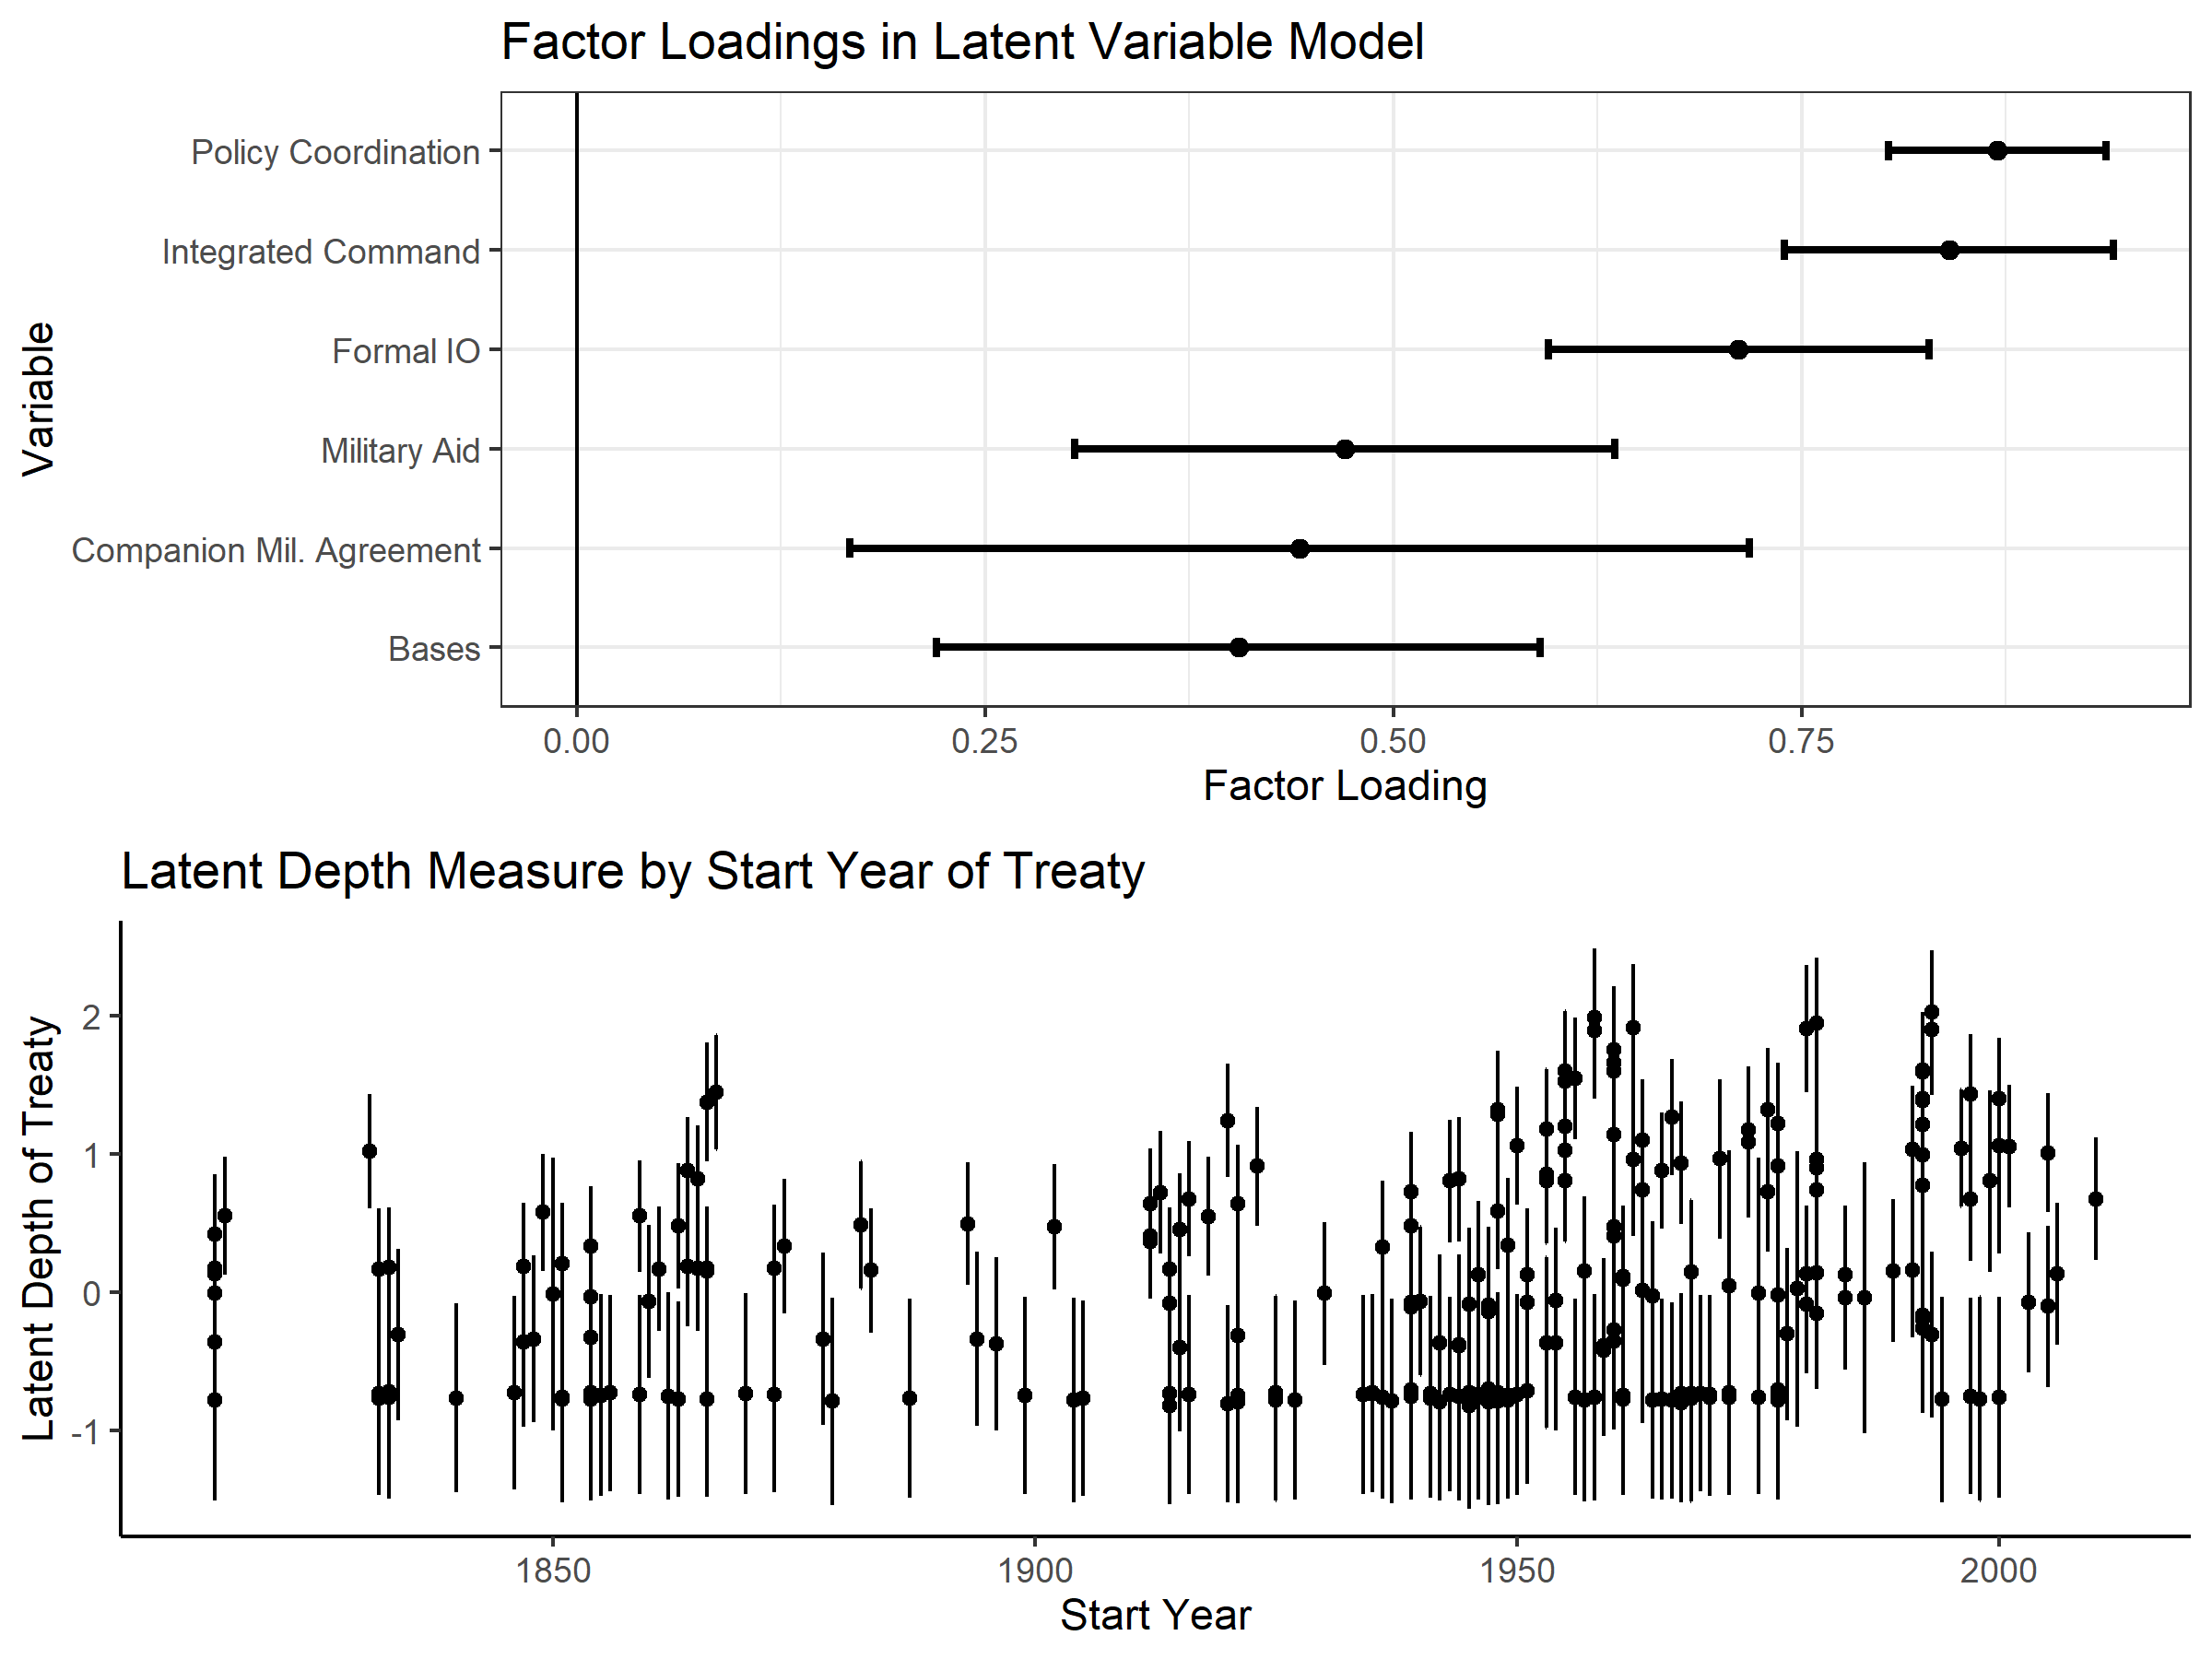
\includegraphics[width=0.95\textwidth]{../figures/loadings-measure.png}
\caption{Factor Loadings and posterior distributions of latent alliance treaty depth measure. Estimates from a semiparametic mixed factor analysis of offensive and defensive ATOP alliances from 1816 to 2007.}
\label{fig:loadings-measure}
\end{figure}


The measurement model predicts each alliance's treaty depth using the factor loadings. 
The bottom panel of \autoref{fig:loadings-measure} summarizes the posterior distributions of the latent treaty depth measure for every alliance in the data. 
There is substantial variation in alliance treaty depth. 
Around half of all formal alliance treaties have some depth, and depth varies widely across alliances.
In the analysis, I measure treaty depth using the mean of the latent depth posterior for each alliance. 
The posterior mean captures the central tendency of latent treaty depth, and I show in the appendix that results are robust to accounting for uncertainty in the latent measure. 


The other outcome variable is a dummy indicator of unconditional military support. 
Using ATOP's information on whether defensive or offensive promises are conditional on specific locations, adversaries, or non-provocation, I set this variable equal to one if the treaty placed no conditions on military support.
123 of 289 alliances offer unconditional military support. 


The key independent variable is an ordinal indicator of open electoral competition in the most capable alliance member in the year of alliance formation. 
I use the Polity2 political institutions data for these measures of democratic institutions and code the alliance leader as the state with the largest CINC score \citep{SingerCINC1988}.\footnote{In some models, I start with an estimate of the most capable alliance members' aggregate Polity score before presenting results with elections, constraints and competition.}
For elections, I use Polity's executive recruitment concept. 
I then use Polity's political competition concept to capture the extent of political competition. 
When the most capable alliance member has both competitive elections and institutionalized open electoral participation, I code the open electoral competition measure as two.
States with either competitive elections or institutionalized electoral participation have a score of one on this ordinal measure. 
When the most capable alliance member has neither elections nor open electoral participation, I set the electoral competition variable to zero.
This measure implies that states with either competitive elections or free political competition have partial electoral scrutiny, while states with both have full electoral competition.\footnote{Results are robust to alternative measures of electoral competition and a measure of the proportion of states with electoral competition which I present in the results section.}
58 alliances have a leader with fully open electoral competition, 14 alliances have partially open competition, and 204 alliances have no meaningful electoral competition in the most capable member. 
This measure emphasizes the influence of the most capable alliance member and operationalizes the potential sensitivity of that state to electoral considerations.   
I also use the Polity data to account for executive constraints.
I set an executive constraints equal to one if the executive constraints concept codes a state as having executive parity or subordination to other branches of government and zero otherwise.



\subsection{Estimation Strategy}


I use several bivariate statistical models to examine how domestic political institutions affect treaty depth for two reasons.\footnote{Bivariate refers to a model means two outcome variables, not a model with only one independent variable.} 
First, my argument expects that the data-generating processes behind treaty depth and unconditional support are related. 
Bivariate estimation also accounts for correlated errors because common unobserved factors may affect depth and conditionality \citep{Braumoelleretal2018}.
This approach emulates the seemingly-unrelated regression model of \citet{FjelstulReiter2019}, who also note that different alliance treaty design decisions are correlated. 
Univariate models assume that alliance treaty design decisions are uncorrelated and if this assumption is violated, these models may produce biased estimates. 
My bivariate model is a generalization of the well-known bivariate probit model, but it is not fully recursive, because I do not include depth or unconditional military support as endogenous predictors.\footnote{A fully recursive model requires instruments for identification.}  
Instead, this model assumes that states make decisions about depth and conditions on military support at the same time. 


To predict unconditional military support, I use a binomial model with probit link function. 
The alliance leader democracy measures are the key independent variables.
Modeling depth is more complicated because the latent measure is skewed.
To facilitate model fitting, I transformed latent depth to range between zero and one and modeled it with a beta distribution.\footnote{I also considered log-logistic, Dagum and inverse Gaussian distributions for the outcome, but AIC and residuals showed that the beta distribution gave the best model fit.}
The flexibility of the beta distribution helps predict mean latent depth.\footnote{Using a beta distribution for the depth outcome also facilitates fitting models that account for uncertainty in the latent measure, which I include in the appendix.} 


In the beta and probit models, I control for several correlates of alliance treaty design and leader institutions. 
Key controls include dummy indicators of asymmetric alliances between non-major and major powers and symmetric alliances between major powers \citep{Mattes2012}\footnote{This leaves symmetric alliances between major powers as the base category for these two binary variables.} as well as the average threat among alliance members at the time of treaty formation \citep{LeedsSavun2007}. 
I also control for foreign policy similarity using the minimum value of Cohen's $\kappa$ in the alliance \citep{Hage2011}.
I draw on the ATOP data \citep{Leedsetal2002}, to adjust for for asymmetric treaty obligations, the number of alliance members and whether any alliance members were at war. 
To capture the role of issue linkages in facilitating alliance agreements \citep{Poast2012}, I include a dummy indicator of whether the alliance made any economic commitments.\footnote{In the appendix, I implement a trivariate model of treaty depth, unconditional military support and issue linkages, because issue linkages also increase treaty credibility \citep{ Poast2013}.}  
Last, I include a count of foreign policy concessions in the treaty, because concessions can facilitate agreement in alliance negotiations \citep{Johnson2015}. 
There is also I also adjust for the role of time and the international context using a smoothed term for the start year of the alliances to capture changes over time.
This captures shifts in the prevalence of deep or unconditional alliances over time.\footnote{Findings about democracy could reflect US alliances. See the appendix for results with an additional control for U.S. membership, which are similar to the inferences below.}


I use a generalized joint regression model (GJRM) \citep{Braumoelleretal2018} to combine the probit and beta specifications in a bivariate model.
This flexible estimator takes the probit and beta models and employs smoothed terms for threat and the start year of the alliance while estimating error term correlations. 
Adjusting for unobserved correlations between depth and unconditional military support ensures accurate inferences about democracy and other covariates.
GJRM uses copulas to model correlated errors in multiple equation models, which makes it more flexible than parametric models and facilitates causal inference. 
Copulas are distributions over functions, and relax potentially problematic assumptions about the shape of the correlation in the error terms. 
Because controlling for correlated errors is crucial for inferences about correlated data-generating processes, considering a range of error distributions should facilitate more accurate inferences. 
I fit models with every possible copula, and selected the best-fitting model using AIC, conditional on that estimator having converged.\footnote{GJRM uses maximum likelihood estimation, and diagnostics for the gradient as well as the information matrix suggest that the models behind all inferences in the paper and appendix converged.} 
The T copula provides the best model fit. 


The argument also provides some insight about variation in how depth and unconditional support are correlated.  
If electoral competition induces leaders to use depth in place of unconditional military support, open electoral competition should encourage negative correlations in the error term. 
Conversely, if executive constraints encourage attempts to precommit successors with costly alliance commitments, constraints should make the error term correlation more positive.
Non-democracies might instead forgo both depth and unconditional support, or form alliances where depth complements unconditional obligations. 
I also suspect that correlations in unobservable factors between treaty depth and unconditional promises of military spending vary with the international context.
For example, \citet{Kuo2019} shows how European politics encouraged the proliferation of secret alliances before World War I, and similar processes of emulation and diffusion may operate over time.
Therefore, I use a third equation in the GJRM estimator to model heterogeneity in the error term correlations, which I expect depends on the start year of the alliance and democratic institutions.
To address the start year of the alliance, I include a smoothed term for the start year of the alliance in the error term equation.  


In summary, the GJRM model is a general and flexible way to simultaneously model different aspects of alliance treaty design.
Like the measurement model, it uses a semiparametric approach to relax potentially problematic assumptions about the distribution of underlying correlations. 
It also allows me to model the two outcomes with appropriate distributions. 
Before presenting inferences from this model, however, I start with descriptive statistics. 
I then use the bivariate model to estimate how electoral competition and executive constraints affect alliance treaty design. 
The next section summarizes the results. 


\section{Results}


My findings are consistent with the claim that competitive elections in the most capable alliance member lead to treaties with conditional support and greater depth. 
Electoral competition increases depth and decreases the probability of unconditional military support.
Executive constraints increase the probability of unconditional military support and decrease treaty depth, however, which is consistent with attempts to precommit successors.
The net effect of democracy still positive for treaty depth and negative for unconditional military support, at least for states with full electoral competition.   


Descriptive statistics are consistent with the two hypotheses.
Treaty depth and electoral competition in the leading alliance member are positively correlated. 
\autoref{fig:democ-combo} shows the average electoral competition among the most capable member when the alliance formed as a function of conditions on military support and treaty depth.
In \autoref{fig:democ-combo}, each quadrant corresponds to a combination of treaty depth and conditionality. 
To create two bins from the continuous latent depth measure, I classified deep alliances as treaties with a latent depth score above the median value. 
Conditional and deep alliances have the highest average electoral competition. 
Conversely, unconditional alliances with little depth have low average electoral competition.


\begin{figure}[hbtp]
\centering
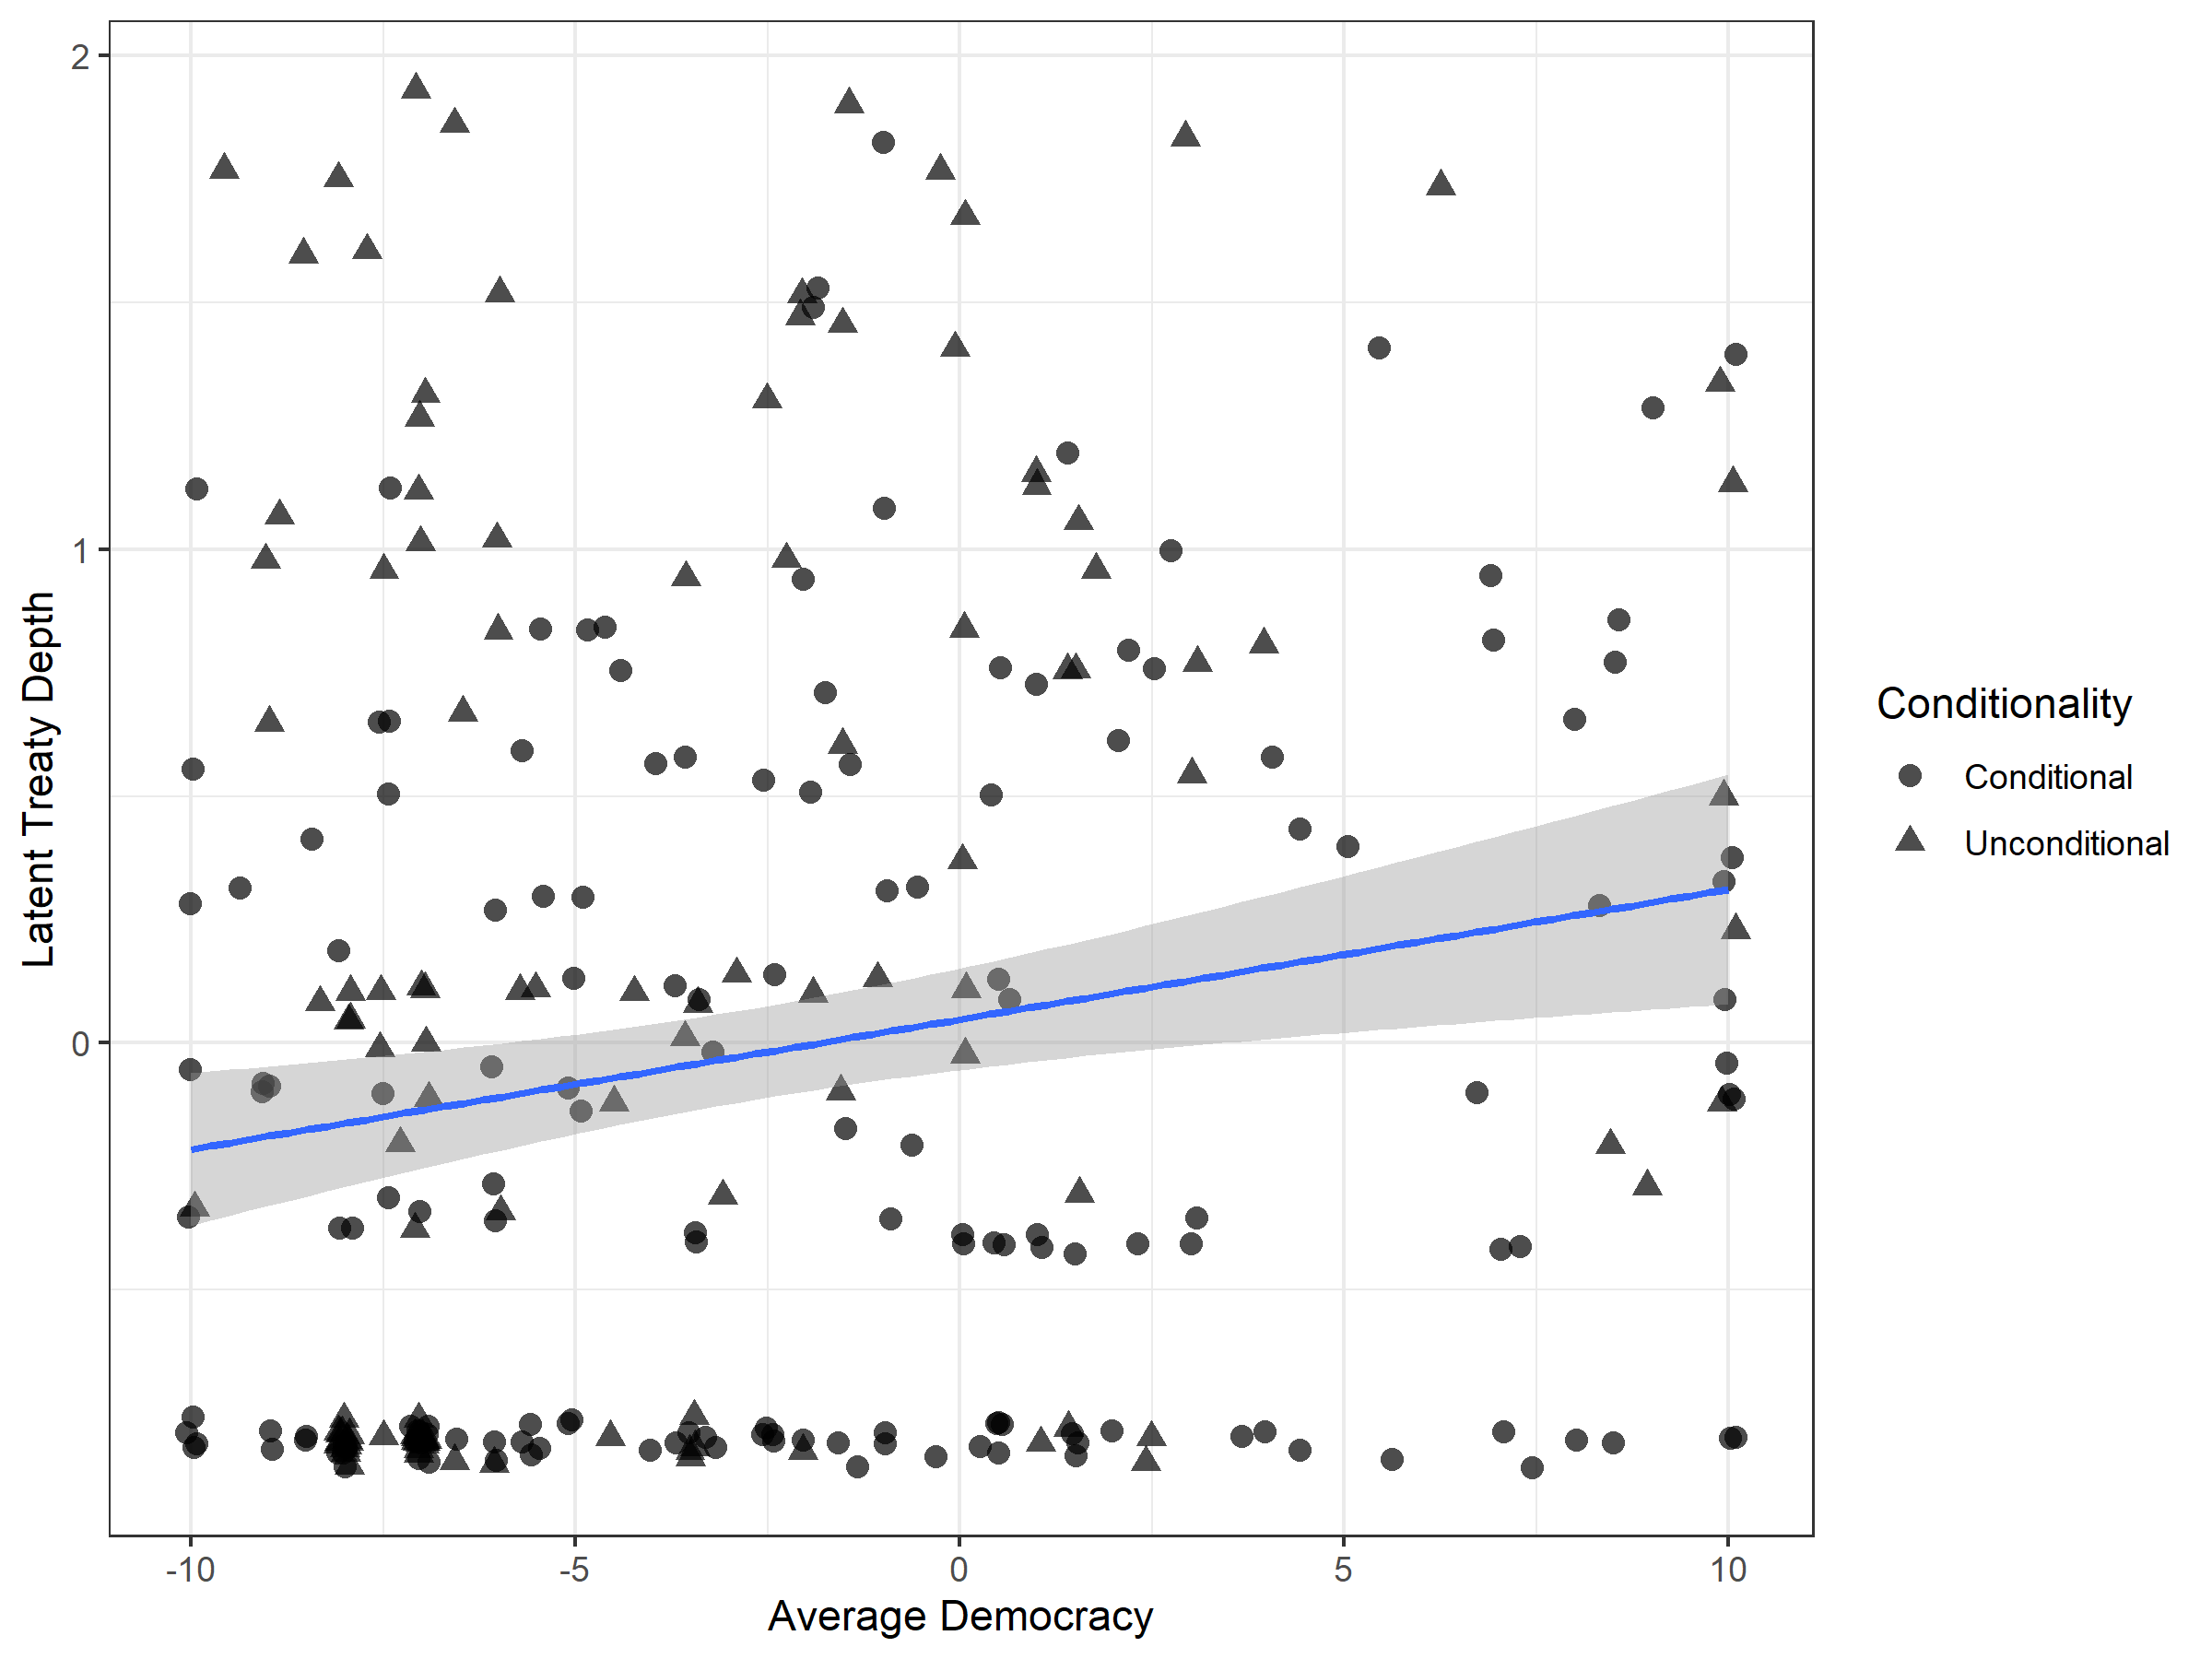
\includegraphics[width=0.8\textwidth]{../figures/democ-combo.png}
\caption{Average extent of electoral cometition within the most capable member at the time of alliance formation across four groups of alliance from 1816 to 2007. Divisions between alliances based on unconditional military support and treaty depth. Darker quadrants mark higher average electoral competition for that group of alliances, and the text in each box gives the precise value.}
\label{fig:democ-combo}
\end{figure}


These descriptive results do not adjust for potential confounding factors, however.
I now report the results of a bivariate model of depth and unconditional military support in \autoref{tab:gjrm-res}. 
This table presents results from both equations of the GJRM.\footnote{I mark smoothed terms with the letter s.} 


\begin{table}[ht]
\centering
\begin{tabular}{lrrrr}
  & \multicolumn{2}{c}{Uncond. Mil. Support} & \multicolumn{2}{c}{Latent Depth}\\ \hline
  & Estimate & Std. Error & Estimate & Std. Error \\ 
  \hline
  Executive Constraints & 0.5023877 & 0.1268535 & -0.1193016 & 0.1128244 \\ 
  Open Electoral Competition & -0.4769550 & 0.1190516 & 0.2595737 & 0.0830853 \\ 
  Economic Issue Linkage & 0.0253785 & 0.1189518 & 0.1706351 & 0.0901450 \\ 
  FP Concessions & -0.1300497 & 0.1088326 & -0.0535896 & 0.0663629 \\ 
  Number of Members & -0.1137716 & 0.0249617 & 0.0308762 & 0.0140311 \\ 
  Wartime Alliances & -0.5924840 & 0.2310503 & -0.1340249 & 0.1425685 \\ 
  Asymmetric Obligations & -0.1578215 & 0.2362376 & 0.1289611 & 0.1541697 \\ 
  Asymmetric Capability & 1.6001969 & 0.4179753 & 0.4474622 & 0.2188766 \\ 
  Non-Major Only & 1.9995336 & 0.4428532 & 0.1419032 & 0.2359317 \\ 
  FP Disagreement & 0.1642942 & 0.2197199 & 0.2019191 & 0.1864040 \\ 
  s(Mean Threat) & 7.8671093 & 113.5851268 & 1.0000063 & 37.8281855 \\ 
  s(Start Year) & 6.1083359 & 122.1899306 & 7.2047971 & 54.4401042 \\ 
  (Intercept) & -1.2256416 & 0.4102588 & -1.3143636 & 0.2559018 \\ 
   \hline
\end{tabular}
\caption{Results from joint generalized regression model of treaty depth and unconditional military support in offensive and defensive alliances from 1816 to 2007. 
                     All smoothed terms report the effective degrees of freedom and the chi-squared term. 
                     The unconditional military support model is a binomial GLM with a probit link function. 
                     The treaty depth model is a beta regression. 
                     I model the error correlation between the two processes with a T copula.} 
\label{tab:gjrm-res}
\end{table}


These estimates are broadly consistent with the argument. 
As electoral competition increases, alliance leaders are more likely to form deep alliances, and less likely to offer unconditional military support. 
Executive constraints has a different effect on alliance treaty design.
First, I find that executive constraints has little impact on treaty depth--- although the coefficient is negative, the direction of the association is unclear.  
Second, domestic institutions with executive parity or subordination increase the probability of unconditional military support.  
Again, executive constraints may encourage democratic leaders to precommit successors with different foreign policy preferences to the alliance. 


The control variables in this model are also interesting.
Asymmetric capability and the number of alliance members both increase depth. 
Asymmetric alliances and symmetric non-major power alliances are more likely to include unconditional military support than symmetric major power alliances. 
I also find that alliances with more members or a member at war when the treaty formed have a lower probability of unconditional military support. 
Last, threat and the year of alliance formation increase unconditional military support and treaty depth, largely in a non-linear fashion.


To assess the substantive impact of elections, I estimated the difference between different institutional situations using simulated coefficients from the model. 
In the scenarios, I held all other variables at their mode or median. 
I then varied open electoral competition and executive constraints. 
\autoref{fig:results-diff} plots the difference in predicted treaty depth or the probability of unconditional military support between four hypothetical alliances and a baseline scenario with no democratic institutions. 
Each scenario includes one of the two non-zero levels of electoral competition and sets executive constraints to zero or one. 


\begin{figure}[hbtp]
\centering
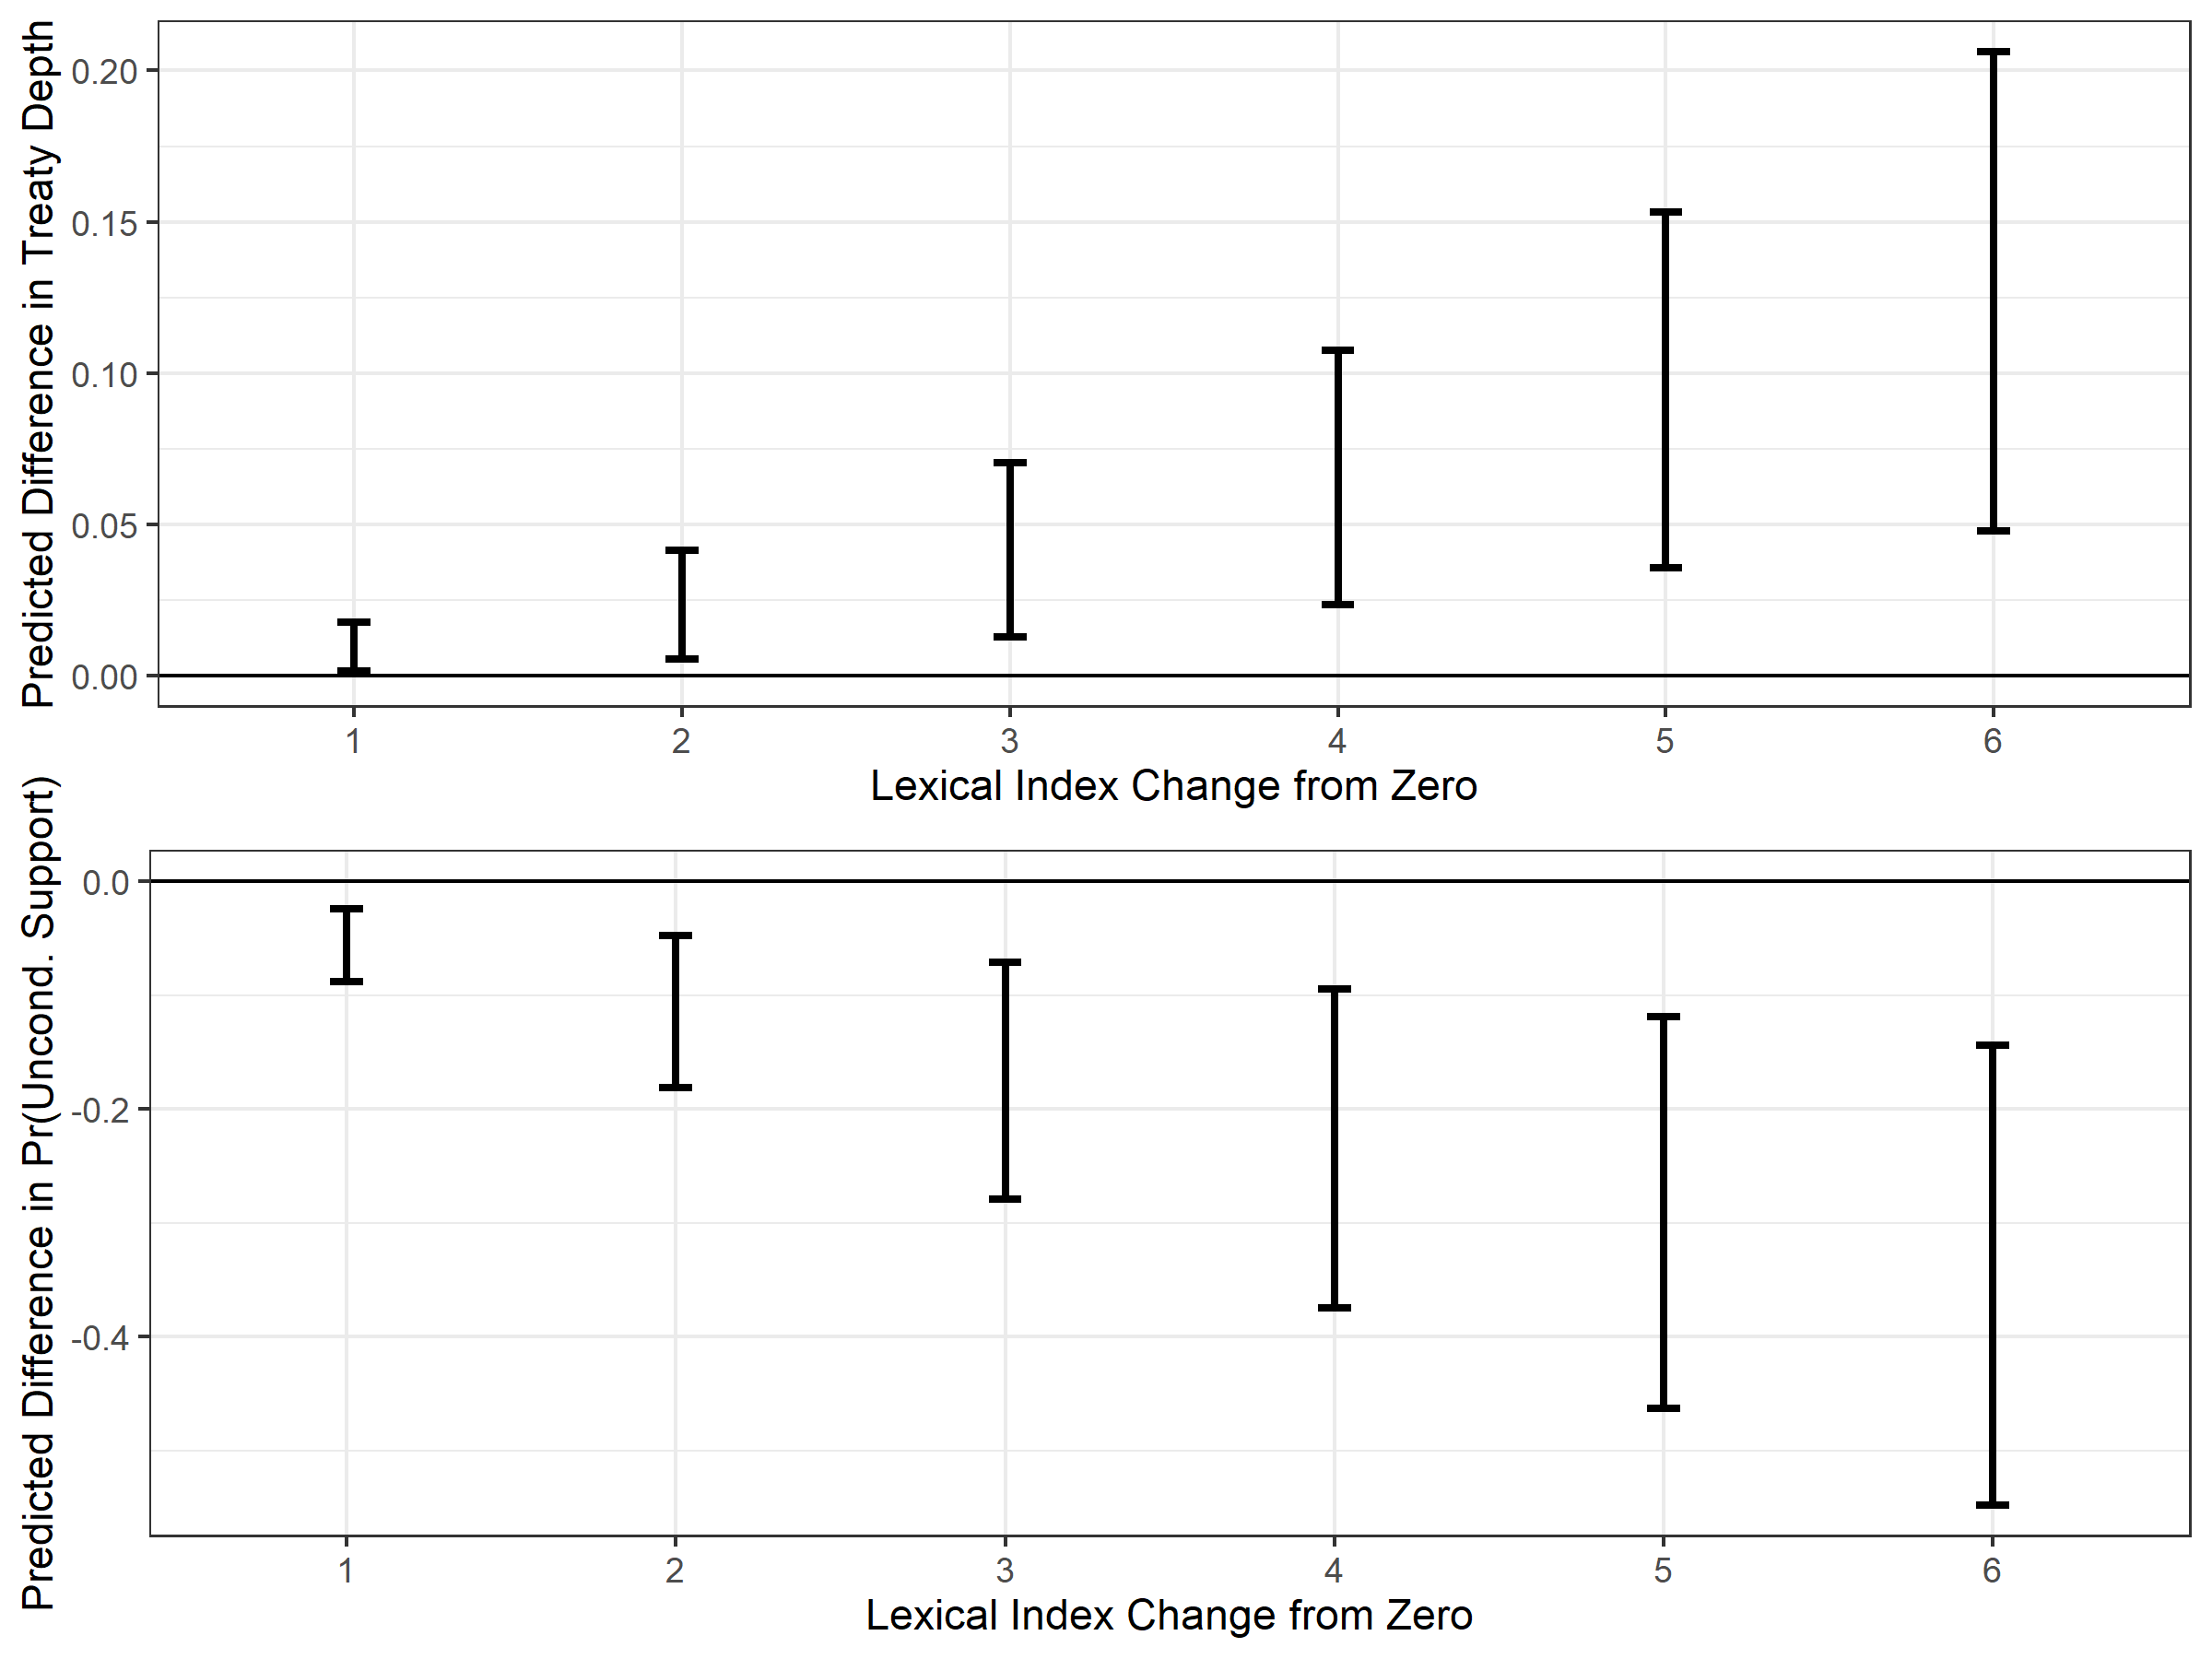
\includegraphics[width=0.95\textwidth]{../figures/results-diff.png}
\caption{Predicted difference in treaty depth and the probability of unconditional military support from a hypothetical alliance where the most capable state has no democratic institutions. The first scenario assesses the impact of adding partial electoral competition. The second scenario assesses the impact of adding full electoral competition. The third and fourth scenarios assess the same changes when executive constraints are present.}
\label{fig:results-diff}
\end{figure}


Partial electoral competition impacts alliance treaty depth and the probability of unconditional military support in states without executive constraints. 
In the absence of executive constraints, partial electoral competition adds between .02 and .09 to treaty depth, and decreases the probability of unconditional military support by between .1 and .25.
Full electoral competition without executive constraints has a larger effect on both depth and unconditional military support. 
As rescaled depth and the probability both range between 0 and 1, these are large effects, though they are based on four and seven observed alliances, respectively. 


Executive constraints attenuate the impact of electoral competition on alliance treaty design, however. 
The overall differences in depth and unconditional support between an alliance leader with executive constraints and limited electoral competition and an alliance leader with neither democratic institution are indistinguishable from zero. 
However, full electoral competition more than offsets the effect of executive constraints on treaty depth.
Alliances where the most capable state has full electoral competition and executive constraints have between .03 and .16 more depth, all else equal. 
The decrease in the probability of unconditional military support is more uncertain, as it ranges between just above zero and -.38. 
These cases with full electoral competition and executive constraints are far more common in the data than the other three scenarios, as there are 51 such observed alliances, which provide a basis for estimating the net impact of full democratic institutions on alliance treaty design.\footnote{These results for democracy and conditions on support are less uniform than those of \citet{Chibaetal2015}. 
The differences are minor, however, as the differences in statistical significance between their democratic proportion variable and the results in \autoref{fig:results-diff} are slight. 
Such small differences between statistically significant and insignificant findings are not themselves statistically significant \citep{GelmanStern2006}, especially in small samples. 
More generally, inferences in small samples are can be more variable.
Given a similar direction of the estimated effects, we draw broadly similar conclusions.}


\autoref{fig:results-diff} shows that the extent of electoral competition affects alliance treaty design.
When alliance leaders face electoral scrutiny, they are more inclined to form deep alliances and add conditions on military support. 
The above results depend in part on correlated errors between depth and unconditional support. 
In the GJRM model, the error term correlations are a function of democratic institutions and the international context. 
I now describe inferences about the error term correlations between treaty depth and unconditional military support. 


As expected, democratic institutions shape the magnitude and direction of the error term correlations between treaty depth and unconditional military support. 
\autoref{tab:error-res} summarizes the estimates from the error term equation, which uses a smoothed term for the start year of the alliance and democratic institutions to predict the unobserved correlations between depth and unconditional military support. 
These estimates are on the scale of a parameter $\theta$ which captures the strength of the association of the errors. 
Competitive elections make the error term correlation more negative, but executive constraints increase it. 
The smoothed term for start years indicates that the relationship between depth and unconditional military support also indicates that the connection between these two facets of alliance treaty design varies widely over time. 


\begin{table}[ht]
\centering
\begin{tabular}{lrrrr}
  \hline
 & Estimate & Std. Error & z value & p-value \\ 
  \hline
Intercept & -1.6162279 & 0.9458270 & -1.7087988 & 0.08748823 \\ 
  Executive Constraints & 4.4235551 & 1.2000196 & 3.6862359 & 0.00022760 \\ 
  Open Electoral Competition & -1.8291556 & 0.6043649 & -3.0265747 & 0.00247342 \\ 
  s(Start Year) & 8.1095245 & 8.6256178 & 54.9617899 & 0.00000001 \\ 
   \hline
\end{tabular}
\caption{Error term correlation equation estimates from a joint generalized regression model of treaty depth and unconditional military support. 
                    Estimates are on the scale of $\theta$, which is then converted into a Kendall's $\tau$ correlation coefficient. 
                    } 
\label{tab:error-res}
\end{table}


The results in \autoref{tab:error-res} suggest that the error term correlation is not a fixed quantity. 
Rather, changes in alliance membership and the international context shape how treaty depth and unconditional military support are connected in alliance treaty design. 
Democratic institutions also have competing effects on the error term correlation, so although elections encourage democracies to substitute depth for unconditional support, executive constraints push in the opposite direction. 


These results use data from the POLITY project. 
Other measures have operationalized electoral competition in other ways, however. 
I now show that my results are largely robust to changing the measure of electoral competition. 


\subsection{Alternative Measures of Electoral Competition}


Some alternative measures of democracy share a similar emphasis on the presence of open and competitive elections. 
As such, these alternative measures should give similar inferences about the connection between democracy and alliance treaty design. 
In this section, I assess two such measures and conceptualize democratic influence in terms of the proportion of alliance members with electoral competition. 


The first measure of electoral competition is the Lexical Index of Electoral Democracy (LIED) \citep{Skaaningetal2015}. 
This ordinal measure assesses the extent of electoral democracy in a country based on six components and ranges from zero to six.  
States with minimally competitive multiparty elections for executive and legislative roles and universal suffrage have the highest possible index score of six.
Other states with partial competition or limited suffrage score lower on this scale. 


The other measure of electoral competition builds off of the concept of polyarchy \citep{Dahl1971}, which includes both contestation and electoral inclusiveness. 
Similarly to my measure, this concept relies on both the opportunity and freedom of actors to compete in elections for leadership. 
States with open political competition and elections for leadership are close to the ideal of electoral democracy, as leaders must address voters' preferences to avoid being removed from office. 
To measure polyarchy, I draw on the polyarchy measure of electoral democracy from the Varieties of Democracy dataset \citep{Teorelletal2016}.


I measure both electoral competition variables in the most capable alliance member in the year the treaty formed. 
I then fit the same bivariate models of treaty depth and unconditional military support as reported above. 
The only change in the models is that I substitute the LEID and polyarchy measures for my ordinal indicator of electoral competition, and change the copulas if needed to maximize model fit.
All of these models include the executive constraints variable from Polity, as this variable is correlated with electoral competition and alliance treaty design. 


As a further check, I translate my electoral competition measure into an alternative conceptualization of democratic influence--- the proportion of democracies in the alliance.
\citet{Chibaetal2015} use the proportion of democracies as their key independent variable, and code this as the share of alliance members with a Polity score above 5 when the alliance formed. 
I expect that the proportion of democracies will also increase alliance treaty depth, as democratic concerns have more weight, and the leading state is more likely to be democratic. 
I express the proportion of democracies as the share of alliance members with a score of one or two on the electoral competition measure. 
I also control for the share of alliance members with executive constraints. 
Because democracies cooperate more with one another \citep{Leeds1999}, the proportion measures are positively correlated with the democratic institutions of the most capable alliance member. 


In \autoref{fig:results-other-democ}, I plot the substantive impact of moving from the minimum to the maximum of the two electoral competition measures and the proportion of alliance members with open competition. 
As in \autoref{fig:results-diff}, these substantive effect calculations hold all other variables in the model constant, and I fix executive constraints to one. 
Each figure in the plot contains three estimates--- the predicted outcome with the key independent variable at its minimum value, the same predictions with the variable at its maximum, and the difference between the two scenarios. 


\begin{figure}[hbtp]
\centering
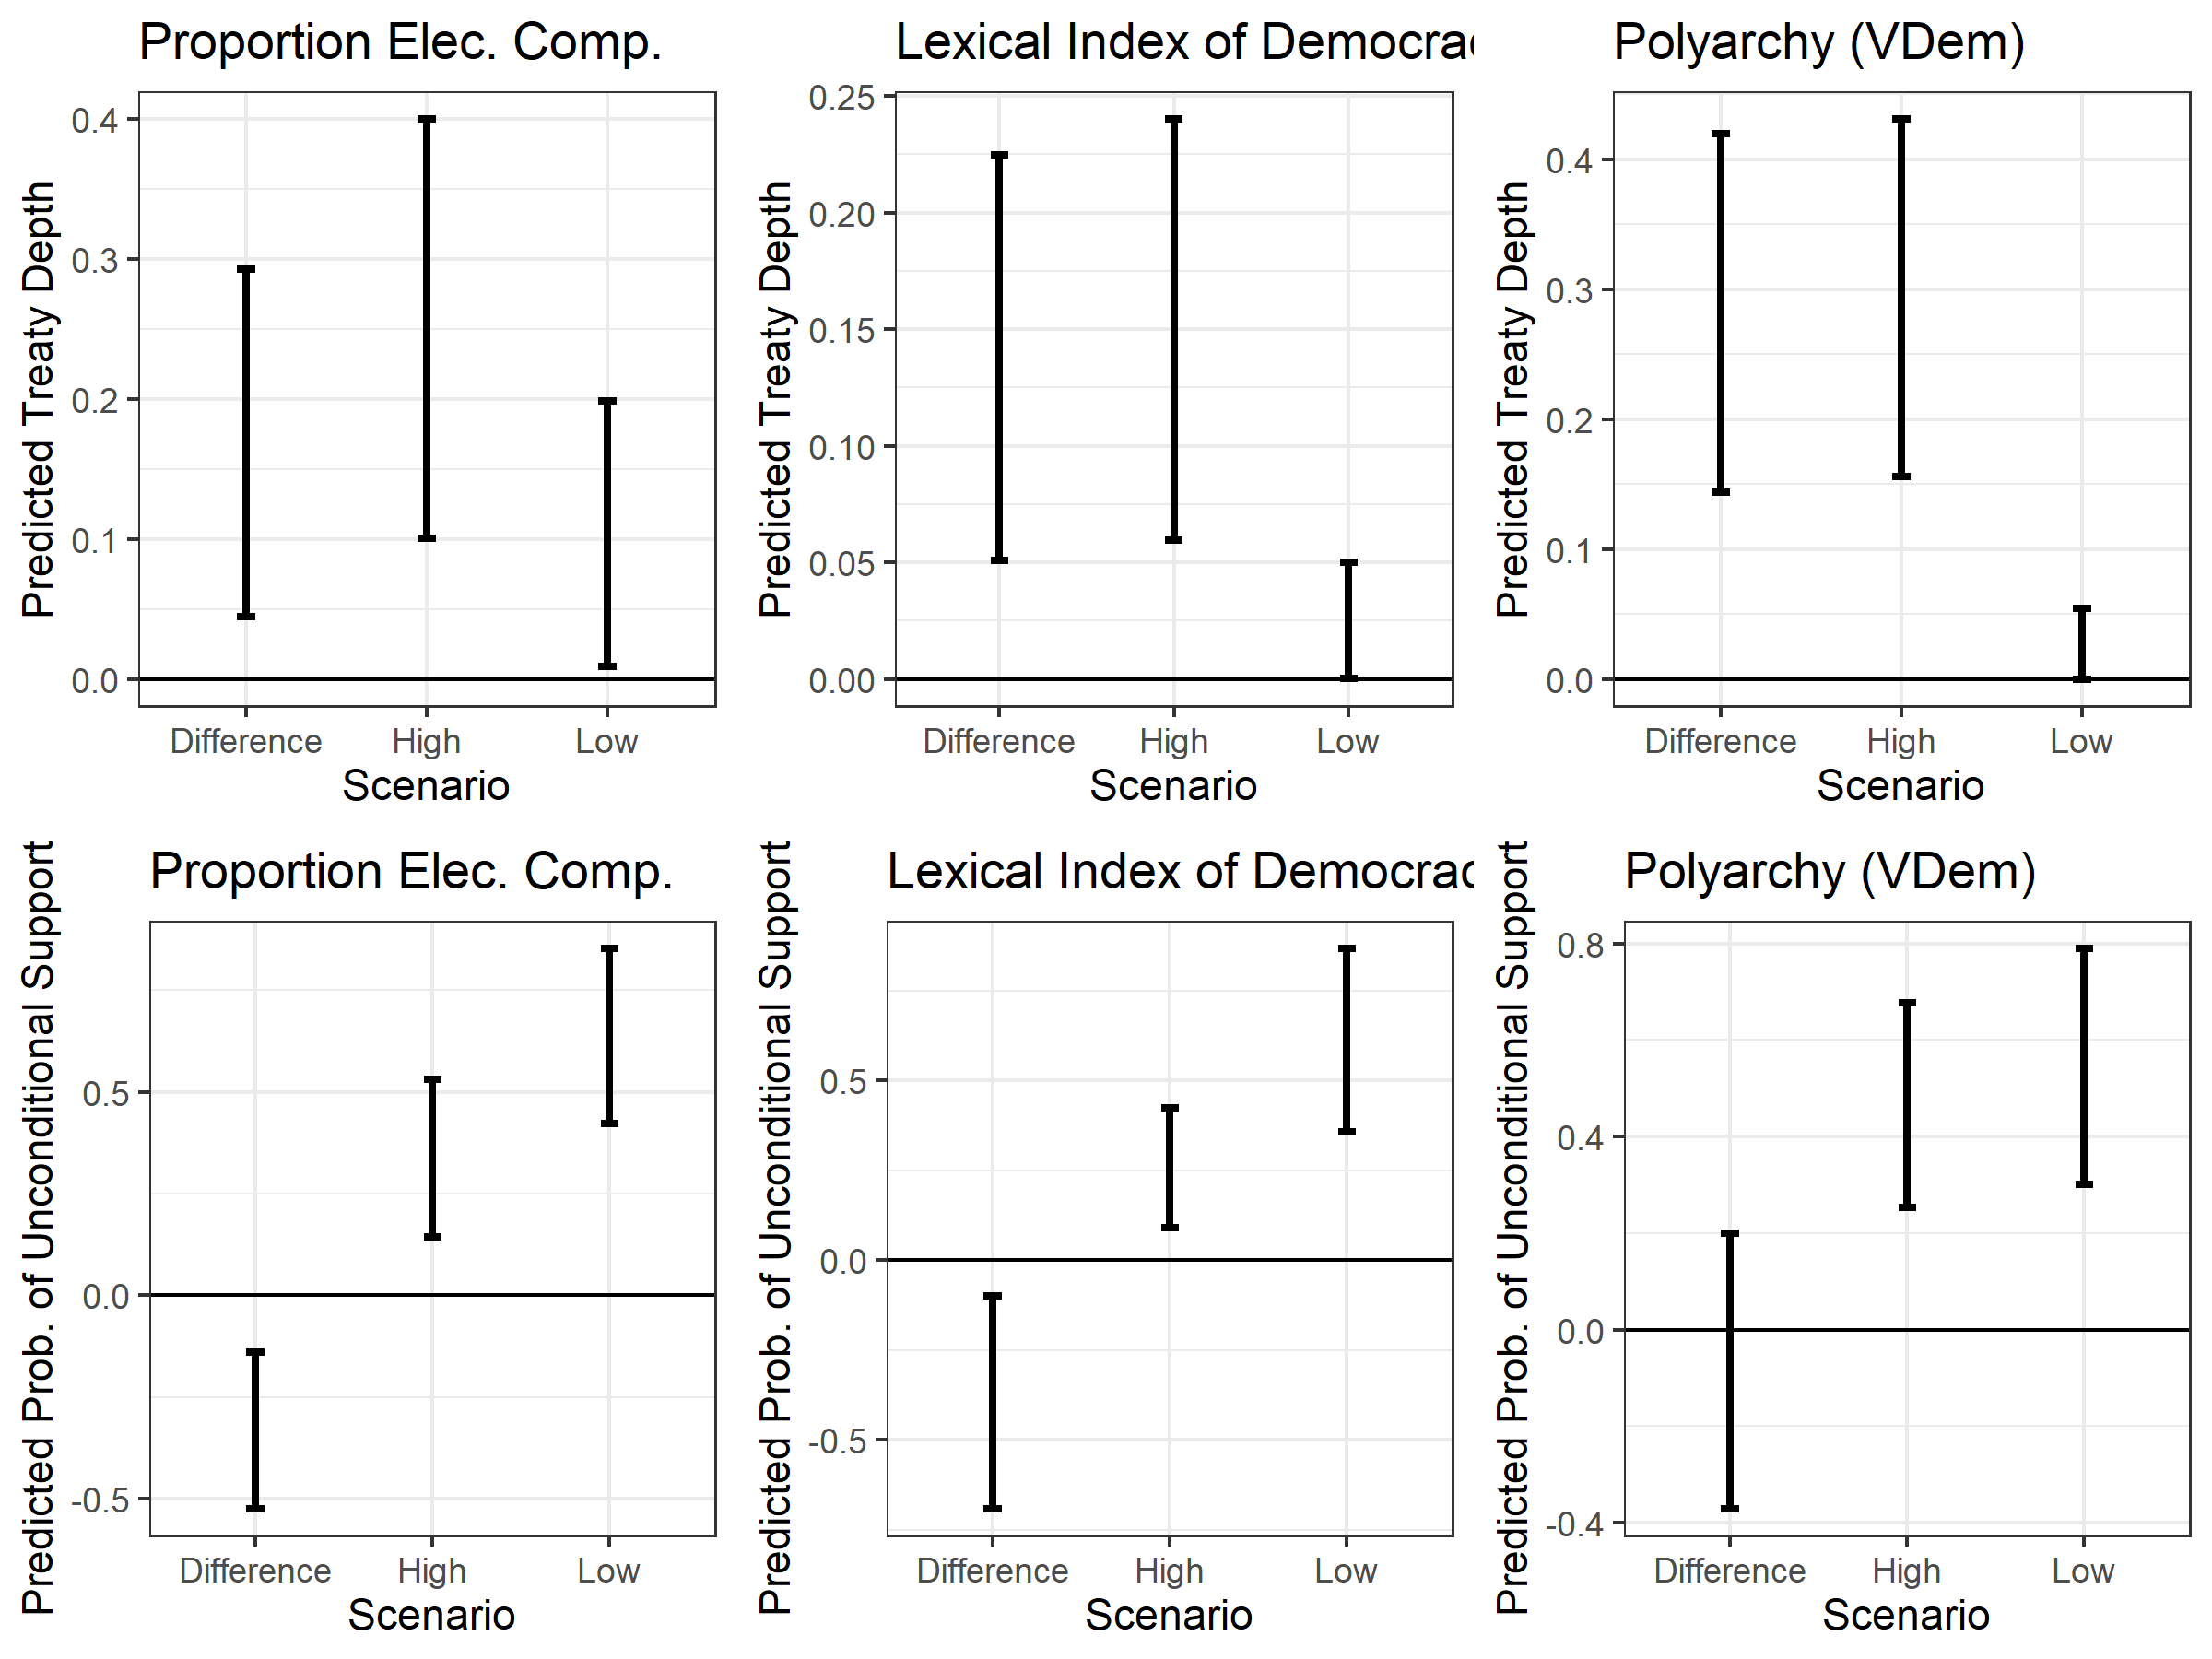
\includegraphics[width=0.95\textwidth]{../figures/results-other-democ.png}
\caption{Predicted treaty depth and probability of unconditional military support in offensive and defensive alliances from 1816 to 2007, all else equal besides an indicator of electoral competition. For each measure of electoral competition, this figure shows the estimated treaty depth or probability of unconditional military support when competition is at maximum or minimum, along with the difference between the two scenarios.}
\label{fig:results-other-democ}
\end{figure}


Results with proportion of alliance members that have open electoral competition match the hypotheses.  
The predicted difference in treaty depth between the low and high extent of electoral competition among alliance members ranges between .05 and .32.
Similarly, more alliance members with competitive elections reduces the probability of unconditional military support by as much as .5, or at least .18. 


Inferences about the association between the LIED and alliance treaty design are also consistent with the argument that elections lead to greater alliance treaty depth.
Moving from no electoral competition to full competition by between .05 and .23, which is a large effect relative to the range of rescaled treaty depth. 
The same shift in electoral competition also reduces the probability of unconditional military support by between .05 and .7. 
So the direction of the effect of greater competition in the LIED is clearly negative, but the magnitude of the effect is uncertain. 


The Varieties of Democracy Polyarchy measure gives slightly different inferences. 
As expected, greater electoral democracy increases treaty depth by between .15 and .43. 
There is no clear difference in the probability of unconditional military support, however.
The polyarchy coefficient behind these substantive estimates is negative, but not clearly so.  
This finding could be explained by the way the Varieties of Democracy project weights the mix of freedom of information and association, along with electoral competition and suffrage, within the polyarchy variable. 
The Varieties of democracy project uses a complicated weighted average that penalizes weaknesses in freedom of information and association for electoral democracy more than other measures. 


The results of these statistical models imply that democratic institutions impact alliance treaty design. 
Electoral competition pushes alliances members to employ treaty depth, rather than unconditional military support.  
Keeping these patterns in mind, I now examine the North Atlantic Treaty Organization (NATO) to illustrate the theoretical process. 


\subsection{NATO Treaty Design}


I use NATO to show the theoretical mechanisms for two reasons. 
First, the process behind NATO applies to multiple alliances, as other US alliance treaties have similar designs. 
Second, NATO is the most important alliance in international politics, as it has played a crucial role in the structure of international relations since 1949. 
Because NATO is an exceptionally durable and consequential alliance, understanding how the treaty formed is worthwhile. 


After World War II, the United States sought a way to protect Europe from the USSR. 
Despite acute security concerns, competition with opposition politicians led the United States to place limits on military support. 
As \citet{Poast2019a} details, NATO members disagreed over how to define the North Atlantic area, especially with reference to France's Algerian colony and Italy, as the North Atlantic area was a key condition on military support. 
Furthermore, active military support from NATO members depends on domestic political processes.\footnote{\citet{Benson2012} calls this commitment a ``probablistic'' obligation.} 
Isolationists in the US Senate feared that an alliance would force America to intervene automatically if partners were attacked, bypassing the power of Congress to declare war and engaging the US in unwanted conflicts \citep[pg. 280-1]{Acheson1969}.
Therefore, Article V of the NATO treaty states that if one member is attacked the others ``will assist the Party or Parties so attacked by taking forthwith, individually and in concert with the other Parties, \emph{such action as it deems necessary} (emphasis mine).'' 
Military support was and is not guaranteed by Article V, and US policymakers used this to sell NATO to the public. 
In a March 1949 press release to the public, Secretary of State Dean Acheson said that Article V ``does not mean that the United States would automatically be at war if one of the nations covered by the Pact is subject to armed attack'' \citep{Acheson1949}.
This claim and the emphases of the press release show that promises of military support were salient to the US public and that entrapment concerns of US leaders led to limited promises of military support. 


Military support from Article V did not assuage European fears that if the Soviets invaded, the United States would not fight. 
To increase the credibility of NATO, the United States took other measures.  
A 1951 presentation by Dean Acheson to Dwight Eisenhower argued that European allies ``fear the inconstancy of United States purpose in Europe. ... These European fears and apprehensions can only be overcome if we move forward with determination and if we make the necessary full and active contribution in terms of both military forces and economic aid'' \citep[pg. 3]{Acheson1951}. 
To start, the US supported the Atlantic Council, an international organization and the main source of depth in the NATO treaty. 
The United States used the Atlantic Council to coordinate collective defense and increase the perceived reliability of the alliance. 
By investing in the Atlantic Council and related joint military planning, the United States addressed European fears of abandonment. 
For example, US officials thought that the British Foreign Minister viewed US provision of a supreme commander in Europe as ``a stimulus to European action'' in NATO \citep{Acheson1950}. 


Policymakers then used defense cooperation with allies to justify NATO participation by arguing that it would facilitate more efficient defense spending. 
In an interview with NBC on March 29, Ambassador at Large Philip Jessup argued that ``One defense program is cheaper and more effective than a dozen national programs. It entails the pooling of information, a joint defense strategy and a pooling of military resources for defense.''
This claim was meant to assuage concerns that NATO would reduce the US ``peace dividend'' after World War II. 


NATO also illustrates that executive constraints might limit treaty depth. 
Many Senators also opposed military aid to Europe \citep[pg 285]{Acheson1969}. 
Thus, legislative constraints on the executive branch reduced the formal depth of NATO relative to what many ambassadors preferred \citep[pg 277]{Acheson1969}, which matches the statistical inference about executive constraints and treaty depth.  
Bilateral agreements on troop deployments thus became another instrument of reassurance. 
In 1950 the Germans formally requested clarification on whether an attack on US forces in Germany would be treated as an armed attack on the United States- and US policymakers said that it would \citep[pg. 395]{Acheson1969}.  
These bilateral arrangements and basing rights are not covered in the NATO treaty, but they added substantial depth.\footnote{This reveals a potential limitation of the statistical models.}  


% Sum up 
In NATO, electoral concerns led the United States to offer conditional military support, but did not inhibit deep military cooperation, which helped reassure European allies. 
Limits on the promises of military support were a salient part of public discussions in the NATO treaty, while the Atlantic Council had a smaller role in public discourse, and policymakers attempted to sell such cooperation as source of efficient defense spending. 
The Atlantic Council and associated bureaucratic machinery are the formal core of substantial defense cooperation. 
NATO negotiations show how a democratic alliance leader used treaty depth to reassure their allies, rather than unconditional military support. 
In the next section, I summarize some implications of the results and offer concluding thoughts. 



\section{Discussion and Conclusion} 


% main evidence summary
In summary, the findings from the statistical models generate consistent evidence for the hypotheses, and the NATO illustration suggests that the theoretical mechanisms are plausible. 
I find consistent evidence that electoral competition drives democracies to design deep alliances.  
Because depth is a less transparent source of alliance credibility, democratic leaders use depth to increase the credibility of alliance commitments, while staying clear of more transparent credibility sources like unconditional military support.
Interestingly, executive constraints increase the probability of unconditional military support, perhaps as it encourages attempts to lock successors into the alliance with unconditional support.
The net effect of democracy on unconditional support is still negative, however, so my results are fairly consistent with previous findings \citep{Mattes2012, Chibaetal2015, FjelstulReiter2019}.  


% limitations
My argument and evidence have two limitations.
First, I only examine variation in formal treaty design. 
This omits treaty implementation, which can diverge from the formal commitment.   
Formal treaty depth often reflects practical depth, but it may miss some differences between alliances. 
Changes in realized alliance depth are a useful subject for future inquiry, but will require extensive data collection.
Second, I examine 280 alliances, so the sample size is limited. 
Inferences from small samples can be more sensitive to model and data changes. 


Shortcomings aside, this paper has three main implications for scholarship. 
First, alliance treaty design is often driven by domestic political considerations. 
Attempts to remain in office and avoid opposition criticism in electoral politics encourage democracies to design deep alliance treaties with conditional promises on military support. 


Second, democracies do not make fully limited alliance commitments. 
A fully limited alliance has conditional obligations and no depth.
Even if democracies impose conditions on military support, treaty depth adds costly obligations, so many democratic alliances are not completely limited.  
Third, some of the lessons from this work might apply to the design on international institutions in general \citep{DownesRocke1995, MartinSimmons1998, Koremenosetal2001, Thompson2010}.
In the same way that democracies use depth to support allies while managing electoral politics, democracies may undertake deep international commitments in ways that limit public scrutiny. 


The findings raise at least two questions for future research.  
For one, they speak to debates about whether democracies make more credible commitments. 
Even if conditional military support reduces the credibility of democratic alliances, treaty depth provides further credibility. 
The net effect of democracy on alliance credibility includes conditions on military support, treaty depth, and the direct effect of democratic institutions and domestic politics. 
These three mechanisms may have competing or conditional effects, which could explain mixed findings about the credibility of democratic commitments \citep{Schultz1999, Leeds1999, Thyne2012, DownesSechser2012, PotterBaum2014}.
Future research should combine the components of democracy and democratic alliances to asses the net effect of democracy on credible commitment in international relations. 


Scholars should also consider how alliance treaty design varies across different types of autocracies. 
The extent and sources of political competition in autocracies varies widely. 
Differences in who selects leaders and what information those actors have about foreign policy \citep{Weeks2008} may help explain alliance treaty design.
For example, personalist leaders with few public or elite constraints on their foreign policy may design alliances with depth and unconditional military support. 


In conclusion, states use deep alliances to reassure their partners while limiting entrapment risk and exposure to audience costs. 
By shaping leaders' foreign policy audiences, domestic political institutions influence how states build credibility into alliance treaties.
Electoral competition encourages democracies to use treaty depth to increase the credibility of their alliances. 



 
\bibliography{../../../MasterBibliography} 





\end{document}
